\chapter{Optimizing Integral Transformations}

\section{A Note on Disk-bound Index Blocking}

The size of tensors grows rapidly in quantum chemistry. The 3-center integrals of density fitting are no exception.
Often, the size of the AO three-index integrals will exceed 64GB of RAM for small systems when
a large basis set such as aug-cc-pVQZ is used, even with sparsity screening. Table 3.1 illustrates this point by listing
the total memory required for sparse three-index AO integrals for the adenine-thymine dimer across various a basis sets. Once the memory required
exceeds what is available, it is necessary for
any implementation to begin reading and writing these tensors to and from disk-based memory. For any field this can
be a major slowdown, but it is especially critical to performance when high-dimensional data is involved. 

\begingroup
\begin{table}[H]
\centering
\renewcommand{\baselinestretch}{1}
\caption{Total memory required for sparse three-index AO integrals for adenine-thymine dimer across various basis sets.
The JK type auxiliary basis sets were used.}
\begin{tabular}{l ccc}
\multicolumn{1}{l}{\textbf{Basis}} &
\multicolumn{1}{c}{\textbf{Memory Required}} &
\multicolumn{1}{c}{\textbf{$N_{AO}$}} &
\multicolumn{1}{c}{\textbf{$N_{aux}$}} \\
\hline

   cc-pVDZ   &      1.0GB    &    321   &     1583\\
aug-cc-pVDZ  &      4.4GB   &     536  &     1986\\
   cc-pVTZ   &      5.4GB    &    724   &     1831\\
aug-cc-pVTZ  &     22.0GB   &    1127  &     2482\\
   cc-pVQZ   &     24.3GB    &   1375   &     2575\\
aug-cc-pVQZ  &     91.4GB   &    2026  &     3534\\
   cc-pV5Z   &     93.3GB    &   2334   &     3687\\
aug-cc-pV5Z  &    316.1GB   &    3293  &     5014\\ 

\end{tabular}
\end{table}
\endgroup

To illustrate
this issue, we will introduce an adapted tensor notation which better indicates memory layout.
We denote an $n$-dimensional tensor as $T_{ab\hdots n}$, where the indices from left to right go from the slowest-running
to the fastest-running indices. Here, $a$ is the slowest-running index, $b$ is the next slowest-running
index, and $n$ is the fastest-running index. The choice of memory layout plays a crucial role when indices are being accessed.
Iterating through the slowest-running index, $a$, would require the largest memory strides whereas the elements 
of the fastest-running index, $n$, are contiguous in memory. 

Now, we can consider two possible forms for the three-center integrals: $A_{P\mu\nu}$ or $A_{\mu P\mu}$.
If these tensors are too large to fit into memory, we must read and write pieces of them to and from disk-based memory.
To accomplish this, we must choose an index to block across. 
For example, if we choose to block across the $P$ index, then we will partition the basis of $P$ into discrete blocks: $P_i \in \{P\}$.
Then, we will read and write only those blocks of $P$ along with all of $\mu$ and $\nu$ for that given block.
The latency of these operations is
bounded by the movement of a physical read-write head, so it is critically important to ensure that read and writes are as
contiguous as possible. In the case of $P$ blocking, the $A_{P\mu\nu}$ tensor is far superior to $A_{\mu P \nu}$ since the 
former will yield entirely contiguous operations whereas the latter will require strided operations. 

Unfortunately, within the density fitting regime, different operations are optimal under different blocking schemes. For example,
consider the construction of the full three-index AO integrals according to (1.9). To accomplish this, 
the initial integrals, $A_{\mu \nu}^P$, are computed and then contracted with the fitting metric. If the AOs are too large to fully 
fit in-core, then we must choose an index, $P$ or $\mu$, to block across. Consider the following two algorithms
that block across either index, respectively:

\begin{algorithm}[H]
\caption{Construct the full AO integrals $B_{\mu \nu}^P$ by blocking across the $P$ index.}
\begin{algorithmic}
\REQUIRE Coulomb metric: $[J]_{PQ}^{-\frac{1}{2}}$
\STATE Initialize: $B_{\mu \nu}^Q$ = 0
\FOR {block $P_i \in \{P\}$}  
    \STATE Compute:  $A_{\mu \nu}^{P_i}$
    \STATE Contract: $A_{\mu \nu}^{P_i} [J]_{P_iQ}^{-\frac{1}{2}} \rightarrow B_{\mu \nu}^Q$
    \STATE Write:    $B_{\mu \nu}^Q$ 
\ENDFOR
\RETURN $B_{\mu \nu}^Q$
\end{algorithmic}
\end{algorithm}

\begin{algorithm}[H]
\caption{Construct the full AO integrals $B_{\mu \nu}^P$ by blocking across the $\mu$ index.}
\begin{algorithmic}
\REQUIRE Coulomb metric: $[J]_{PQ}^{-\frac{1}{2}}$
\FOR {block $\mu_i \in \{\mu\}$}  
    \STATE Compute:  $A_{\mu^i \nu}^{P}$
    \STATE Contract: $A_{\mu^i \nu}^{P}[J]_{PQ}^{-\frac{1}{2}} \rightarrow B_{\mu_i \nu}^Q$
    \STATE Write:    $B_{\mu_i \nu}^Q$
\ENDFOR
\RETURN $B_{\mu \nu}^Q$
\end{algorithmic}
\end{algorithm}

Of the two algorithms, only Algorithm 4 would respect the memory constraints of a blocking procedure. Note that after the 
contraction $A_{\mu \nu}^{P_i} [J]_{P_iQ}^{-\frac{1}{2}} \rightarrow B_{\mu \nu}^Q$ in Algorithm 3, the full 3-dimensional quantity
$B_{\mu \nu}^Q$ is returned, which would immediately violate memory constraints. For this operation, only one blocking method is
\textit{possible}. If we are constrained to blocking across the $\mu$ index, then the tensor form $A_{\mu P \nu}$ will yield
superior disk performance, as it would allow for completely contiguous read operations. The purpose of this illustration is
to remind the reader that for large enough systems, disk performance
is crucially important, therefore memory layout should be considered carefully.

\section{Memory Layout for Sparsity-utilized Transformations}

Algorithm 2 revealed a technique that can be used to utilize sparsity when carrying out three-index integral transformations.
Although utilizing sparsity is imperative for cost reduction, an optimal implementation must be tailored to
fully exploit modern computing hardware.
Multi-core processors consisting of upwards of ten cores are found commonly both at the desk of computational
chemists and in commodity computing clusters.
Moreover, the birth of Intel's manycore architecture , and the advent of Graphics Processing Units (GPUs), 
further necessitate that scientific computing
exploit every means of parallelism.
Although the density fitting technique has been shown to be challenging to exploit in massively parallel
algorithms \cite{ref3}, it remains an essential technique for accelerating computations of 
small to intermediate size chemical systems.
The communication overhead that hinders large scale parallelism for density
fitting is nominal for single node investigations, but even a single multi-core processor contains viable
parallelism that can be challenging to fully exploit. 
Coupling the cost reduction of sparsity approximations with a finely tuned parallel code is crucial to performance.  

Maximizing parallelism in Algorithm 2 will require careful implementation design. 
The choice of memory layout for the sparse 3-dimensional integral tensors will affect both algorithmic 
complexity and parallel scalability. For the three-center integrals, we use $A_{P\mu \nu}$ to denote a memory 
layout with the auxiliary index $P$ as the slowest-running index. 
The $A_{P \mu \nu}$ layout is intuitive, as it allows looping through $P$ and direct application sparsity mask 
for each submatrix. The resulting sparse form $A_{P \mu \nu^\mu}$ contains submatrices of identical structure.
However, another form, $A_{\mu P \nu}$, must be considered. The sparse form $A_{\mu P \nu^\mu}$
results in submatrices of differing sizes. However, some advantages may be ascertained.
We sought to determine which of these two sparse memory layouts, $A_{P \mu \nu^\mu}$ or 
$A_{\mu P \nu^\mu}$, is optimal for transforming the integrals into an MO basis.
Algorithms 5 and 6 illustrate the difference:

\begin{algorithm}[H]
\caption{Transforming sparse integrals using $A_{P \mu \nu^\mu}$ form.}
\begin{algorithmic}
\REQUIRE Sparse AO integrals: $A_{P \mu \nu^\mu}$, orbital matrices: $C_{\mu p}, C_{\nu q}$, screening mask: $S_{\mu \nu}^b$
\FOR {$P = 0$ to $P = N_{aux}-1$}
    \FOR {$\mu = 0$ to $\mu = N_{AO}-1$}  
        \STATE Trim from dense to sparse: $C_{\nu q}S_{\mu \nu}^b \rightarrow C_{\nu^{\mu} q}$
        \STATE $A_{P \mu \nu^\mu} C_{\nu^{\mu} p} \rightarrow A_{P \mu p}$
    \ENDFOR
\ENDFOR
\RETURN $A_{P \mu p}$
\STATE Final transform: $A_{P \mu q}C_{\mu p} \rightarrow A_{P p q}$
\RETURN $A_{P p q}$
\end{algorithmic}
\end{algorithm}

\begin{algorithm}[H]
\caption{Transforming sparse integrals using $A_{\mu P \nu^\mu}$ form.}
\begin{algorithmic}
\REQUIRE Sparse AO integrals: $A_{\mu P \nu^\mu}$, orbital matrices: $C_{\mu p}, C_{\nu q}$, screening mask: $S_{\mu \nu}^b$
\FOR {$\mu = 0$ to $\mu = N_{AO}-1$}  
    \STATE Trim from dense to sparse: $C_{\nu q}S_{\mu \nu}^b \rightarrow C_{\nu^{\mu} q}$
    \STATE $A_{\mu P \nu^{\mu}} C_{\nu^{\mu} q} \rightarrow A_{\mu Pq}$
\ENDFOR
\RETURN $A_{\mu P q}$
\STATE Final transform: $A_{\mu P q}C_{\mu p} \rightarrow A_{p P q}$
\RETURN $A_{p P q}$
\end{algorithmic}
\end{algorithm}


To carry out the first step of the transformation, both algorithms must loop through the slowest-running index of the integrals.
Operations within this loop should be parallelized.
The number of iterations for this step are greater in Algorithm 3 than in Algorithm 4 since $N_{aux}$ will always be 
larger than $N_{AO}$.
Conversely, the matrix-matrix multiplications occurring in Algorithm 4 are larger. As a result, Algorithm 4 will benefit from delegating
larger problem sizes to highly optimized level 3 BLAS routines. 

However, the crucial difference is ascertained when one considers which index, $\mu$ or $P$, would be most appropriate to block across
for a disk-bound implementation. If we choose to block across $\mu$, the result of the final transformation, $A_{pq}^P$, would be incomplete,
and a full cumulative disk write of $\mathcal{O}(N_{aux}N_pN_p)$ size would be necessary for each block of $\mu$. Moreover, there is a chance
this operation could be altogether impossible if memory constraints would be violated by having a full $A_{pq}^P$ tensor in memory. 
On the other hand, 
blocking across the $P$ index would not pose this problem, as no contractions occur across the $P$ index. Therefore, blocking across 
$P$ is the only scalable solution.

Now, if it is necessary to block across $P$, consider the implications for Algorithms 5 and 6. For Algorithm 5, this means that if the blocks
over $P$ are very small, e.g. $<10$, then the parallelized loops will have very few iterations. Typically, the fewer the iterations the worse
the parallel scalability as the workloads are much more susceptible to being unbalanced. To the contrary, Algorithm 6 will not suffer this 
drawback and is therefore the better option. Since Algorithm 6 contains higher concurrency and utilizes larger matrix-matrix multiplications, 
we propose that it will yield enhanced parallel scaling. 

\section{Context Dependent Workflows}

Equation (1.9) demonstrates the necessity of the fitting metric when using the 3-center density-fitted integrals. Unfortunately, the
metric contraction in equation (1.9) comes at the heavy price of $\mathcal{O}(N_{aux}^2N_{AO}^2)$ operations.
Considering that $N_{aux}$ can be 2-3x larger
than $N_{AO}$, this can be an extremely costly operation. One remedy for cost reduction is to transform the 3-center integrals prior to contracting
them with the metric:
\begin{align} 
A_{p q}^Q &= A_{\mu \nu}^Q C_{\mu p}C_{\nu q} \\
B_{pq}^P &= [J]_{PQ}^{-\frac{1}{2}}A_{p q}^Q
\end{align}
 
\noindent Since $N_p$ and $N_q$ are often much smaller than $N_{AO}$, the speedup of 
$\mathcal{O}(\frac{N_{AO}^2}{N_pN_q})$ can be substantial. 
Table 3.2 illustrates the potential benefit for some commonly used transformed integrals using occupied and virtual spaces.
Orbital indices $i,j$ denote occupied spaces and $a,b$ denote virtual spaces.

\begingroup
\begin{table}[H]
\centering
\renewcommand{\baselinestretch}{1}
\caption{Speedups obtainable via pre-transforming the 3-center integrals prior to metric contraction for common occupied-virtual transformations.
$N_{AO}$ and $N_i$ denote the number of atomic orbitals and occupied molecular orbitals, respectively. }
\begin{tabular}{l c c c}
\multicolumn{1}{l}{\textbf{Transformation}} &
\multicolumn{1}{c}{\textbf{$\frac{N_{AO}}{N_i}=2$}} & 
\multicolumn{1}{c}{\textbf{$\frac{N_{AO}}{N_i}=5$}} & 
\multicolumn{1}{c}{\textbf{$\frac{N_{AO}}{N_i}=10$}} \\ 
\hline
$(Q|ij)$       & 4               & 25              & 100      \\ 
$(Q|ia)$       & 4               & 6.25            & 11.1     \\ 
$(Q|ab)$        & 4              & 1.56            & 1.23     \\
\end{tabular}
\end{table}
\endgroup

The speedups in Table 3.2 are undoubtedly beneficial and this technique is commonly used in practice. 
However, we propose that this technique will be a disadvantageous in certain contexts. 
Namely, applying this workflow to methods using many transformations will increase cost unnecessarily. 
Using this method, a metric contraction is necessary for each transformation, whereas only one contraction is required if this technique is not used.
If many transformations occur, the cost of contracting the metric for 
each transformation will eventually outweigh the speedups attainable in Table 3.2. Therefore, both workflows must be considered when carrying
out 3-center integral transformations. Algorithm 7 and 8 illustrate the corresponding workflows:

\begin{algorithm}[H]
\caption{The "Store" algorithm - contract metric then transform.}
\begin{algorithmic}
\REQUIRE AO integrals: $A_{\mu \nu}^P$, fitting metric: $[J]_{PQ}^{-\frac{1}{2}}$, orbital matrices: $C_{\mu p}, C_{\nu q}$
\STATE Contract metric: $A_{\mu \nu}^P [J]_{PQ}^{-\frac{1}{2}} \rightarrow B_{\mu \nu}^Q$
\STATE Save: $B_{\mu \nu}^Q$
\FOR {all transformation spaces: $C_{\mu p}, C_{\nu q}$}  
    \STATE Transform: $B_{\mu \nu}^QC_{\mu p}C_{\nu q} \rightarrow B_{p q}^Q$
\ENDFOR
\RETURN $B_{p q}^Q$
\end{algorithmic}
\end{algorithm}

\begin{algorithm}[H]
\caption{The "Direct" algorithm - transform then contract metric.}
\begin{algorithmic}
\REQUIRE AO integrals: $A_{\mu \nu}^P$, fitting metric: $[J]_{PQ}^{-\frac{1}{2}}$, orbital matrices: $C_{\mu p}, C_{\nu q}$
\STATE Compute: $A_{\mu \nu}^Q$
\FOR {all transformation spaces: $C_{\mu p}, C_{\nu q}$}  
    \STATE Transform: $A_{\mu \nu}^PC_{\mu p}C_{\nu q} \rightarrow A_{p q}^P$
    \STATE Contract metric: $A_{p q}^P [J]_{PQ}^{-\frac{1}{2}} \rightarrow B_{p q}^Q$
\ENDFOR
\RETURN $B_{p q}^Q$
\end{algorithmic}
\end{algorithm}

\noindent Hereafter we refer to the Store algorithm being the workflow that contracts the metric and then transforms the integrals. Conversely, 
we refer to the Direct algorithm as the workflow that transforms the integrals then contracts the metric. 

Depending on the context, either the Store or Direct algorithm may be superior. We propose the Store algorithm 
will be superior for procedures requiring
many transformations. This includes contexts which iteratively recompute transformations, such as density-fitted 
multiconfigurational self-consistent field (DFMCSCF) \cite{Hohenstein:2015:224103}, 
as well as contexts 
involving a large number of transformations spaces, such as density-fitted symmetry-adapted perturbation theory (SAPT) \cite{ref6, ref7}. 
Conversely, the Direct algorithm will be superior in contexts requiring a small number of transformations. Most notably, 
this includes density-fitted second-order M{\o}ller-Plesset perturbation theory (DFMP2) \cite{ref4}.

%
%\section{Disk IO considerations for transformed integrals}
%Remember that the transformed integrals, $A_{pq}^P$, are used within the context of varous density-fitted proocedures, such as M\{o}ller-Plesset
%Perturbation Theory (DFMP2), Multi-configurational Self-Consistent Field (DFMCSCF), Electron Propagator Theory (DFEP2), and many more.
%Depending on the implementation, these procedures could use one of three memory layouts: $A_{Ppq}$, $A_{pPq}$, or $A_{pqP}$. 

\section{Intermediate Recycling}

Quantum chemistry procedures can require numerous integral transformations. For example, an unrestricted Hartree-Fock (UHF) based SAPT
procedure will employ
24 unique integral transformations. Since all transformations are carried out at the same stage of the computation, one should build an 
implementation that queues the transformations, gathers information, and deploys strategic contraction paths.
As mentioned previously, the first contraction of these integral transformations $A_{p \nu}^P=A_{\mu \nu}^PC_{\mu p}$ 
should always be carried out on the smallest MO index $p$ 
possible. Thereafter, transformations using the same intermediate, $A_{p \nu}^P$, should all occur at the same time to avoid
recomputing $A_{p \nu}^P$. 
For example, suppose two sets of transformed integrals are required, $A^P_{u v}$ and$A^P_{up}$, where $u,v << N$ are
indices restricted to some small "active" subspace of MOs
and $p$ is a general MO index where $N_p \approx N_{AO}$. For both transformations, the first step will be:
\begin{align} 
A^P_{\mu \nu}C_{\mu u} \rightarrow A^P_{u \nu} 
\end{align}

\noindent If this is recognized beforehand, then this operation need only be carried out once and 
the intermediate $A^P_{u \nu}$ can be recycled
for both transformations. The speedup of doing so is $\mathcal{O}(\frac{2N_{AO} + N_v + N_p}{N_{AO} + N_v + N_p})$, 
which as $N_p \rightarrow N_{AO}$ approaches
50\%. Although the benefit is modest, it must be considered for optimized procedures.

\section{Results}

All methods were implemented in the {\sc Psi4} electronic structure software package \cite{Parrish:2017:3185}.
The parallelism in {\sc Psi4} relies on the shared memory programming model using OpenMP 
and carries out matrix multiplications using Intel's Math Kernel
Library. 


\subsection{Parallel Scaling of Transformations}

To measure parallel scaling, we performed integral transformations for the boron catalyst system shown in Figure 3.1. 
We varied the problem size by adjusting the $\zeta$ level for the Dunning correlation-consistent basis sets with $\zeta$ = D, T, Q.
The characteristics of these systems are included in Table 4. Note that while parallel scaling typically improves
for larger systems (i.e. due to larger workloads),
this is not guaranteed in a sparsity regime. Larger systems may contain more sparsity;
more sparsity will result in more striding, copying, and irregular sizing,
which will hinder parallel scaling. Nonetheless, our method outlined in Algorithm 2 is designed to utilize sparsity while also
obtaining maximum parallel efficiency. 

\begin{figure}[H] 
\centering
\includegraphics[width=80mm]{geometries/boron_catalyst.png} \caption{Transition state for organoboron addition to trifluooroacetone. Taken from Ref. \cite{Lee:2016}} 
\label{fig:databases} \end{figure}

\begingroup
\begin{table}[H]
\centering
\renewcommand{\baselinestretch}{1}
\caption{Characteristics of organoboron catalyst.
$N_{AO}$ and $N_{aux}$ refer to the number of primary and auxiliary basis functions, respectively.
Mask sparsity refers to the percentage of significant AO function pairs in the sparsity mask.}
\begin{tabular}{l ccc}
\multicolumn{1}{l}{\textbf{Basis}} &
\multicolumn{1}{c}{\textbf{$N_{AO}$}} &
\multicolumn{1}{c}{\textbf{$N_{aux}$}} &
\multicolumn{1}{c}{\textbf{Mask Sparsity (\%)}} \\
\hline
cc-pVDZ   & 671  & 3277 & 29.6 \\          
cc-pVTZ   & 1566 & 3856 & 41.1 \\          
cc-pVQZ   & 3040 & 5593 & 50.2 \\          
\end{tabular}
\end{table}
\endgroup


\noindent For each system, we performed the three common transformations:

\begin{align} 
(i j | Q) = (\lambda \sigma | Q) C_{\sigma i} C_{\lambda j} , \\
(i b | Q) = (\lambda \sigma | Q) C_{\sigma i} C_{\lambda b} , \\
(a b | Q) = (\lambda \sigma | Q) C_{\sigma a} C_{\lambda b} , 
\end{align}

\noindent where $i$ and $j$ refer to occupied orbitals, and $a$ and $b$ refer to unoccupied orbitals.
The experiment was carried out using one node consisting of an Intel Xeon E5-2630 processor 
(10 cores at 2.20GHz) and using 24GB DRAM. Figure 4 includes plots of both speedups and execution times for each system.

\begin{figure}[H]
  \centering
  \subfloat[]{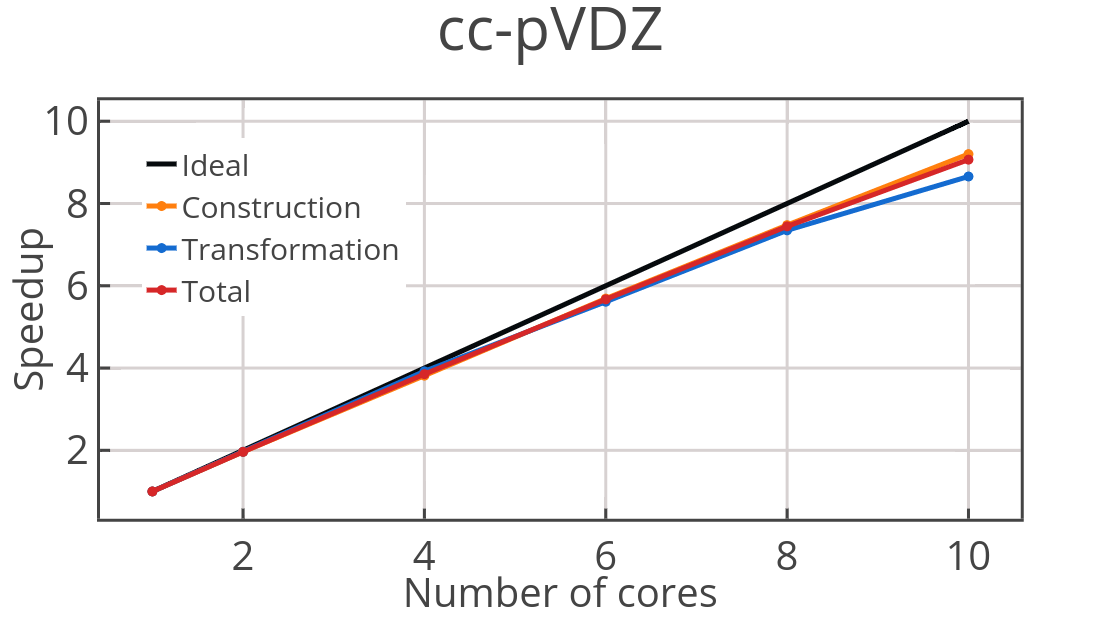
\includegraphics[width=0.5\textwidth]{figures/parallel_scaling_plots/speedup-cc-pVDZ.png}\label{fig:f1}}
  \hfill
  \subfloat[]{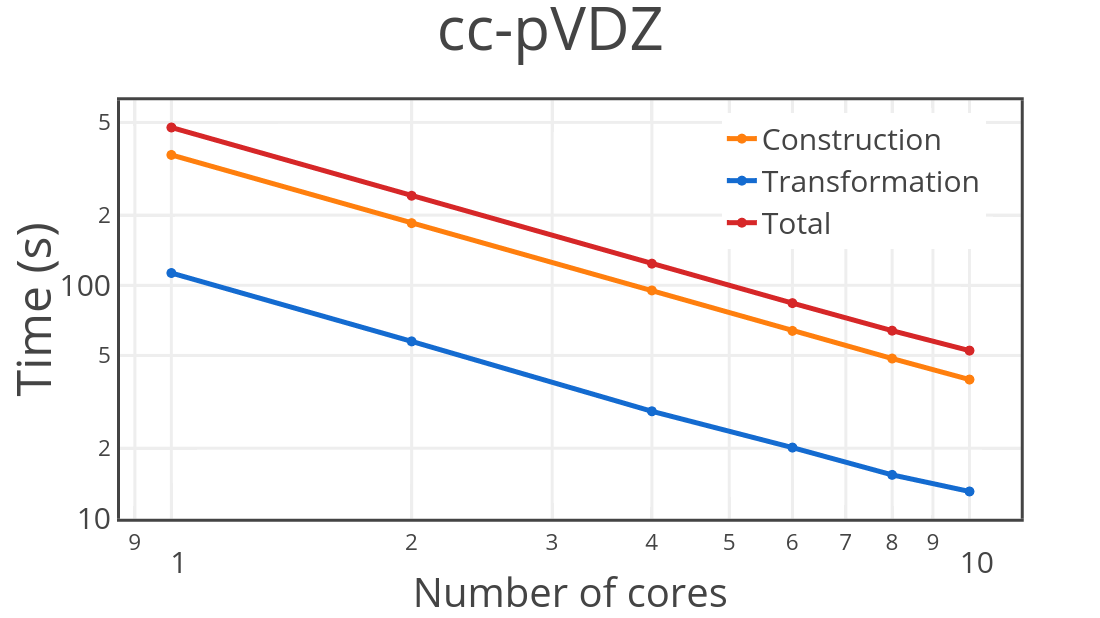
\includegraphics[width=0.5\textwidth]{figures/parallel_scaling_plots/times-cc-pVDZ.png}\label{fig:f2}}
  \hfill
  \subfloat[]{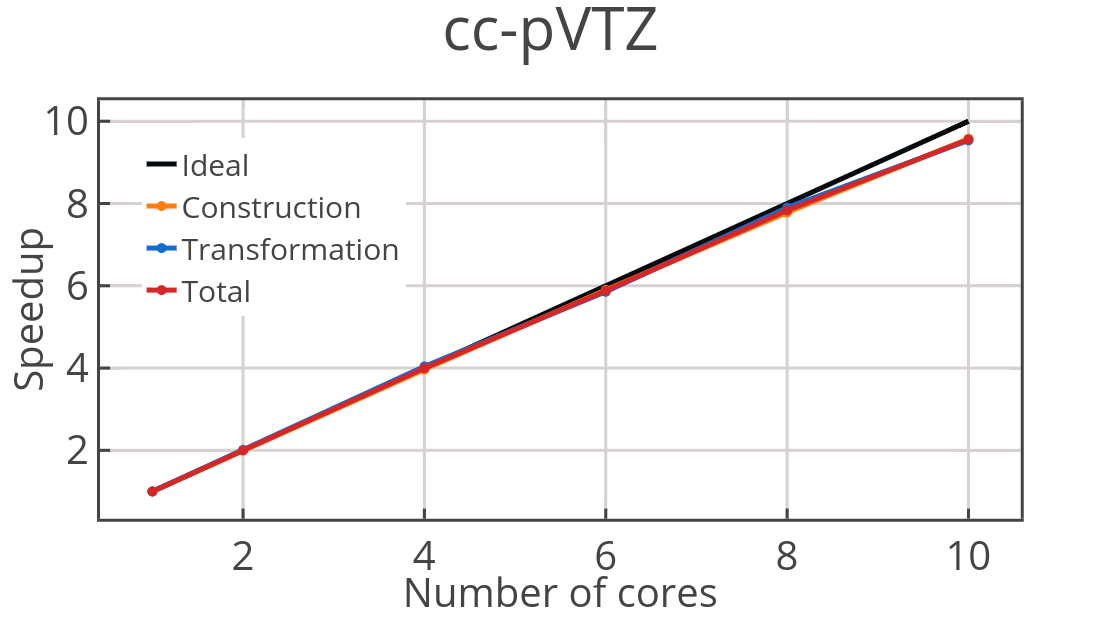
\includegraphics[width=0.5\textwidth]{figures/parallel_scaling_plots/speedup-cc-pVTZ.png}\label{fig:f1}}
  \hfill
  \subfloat[]{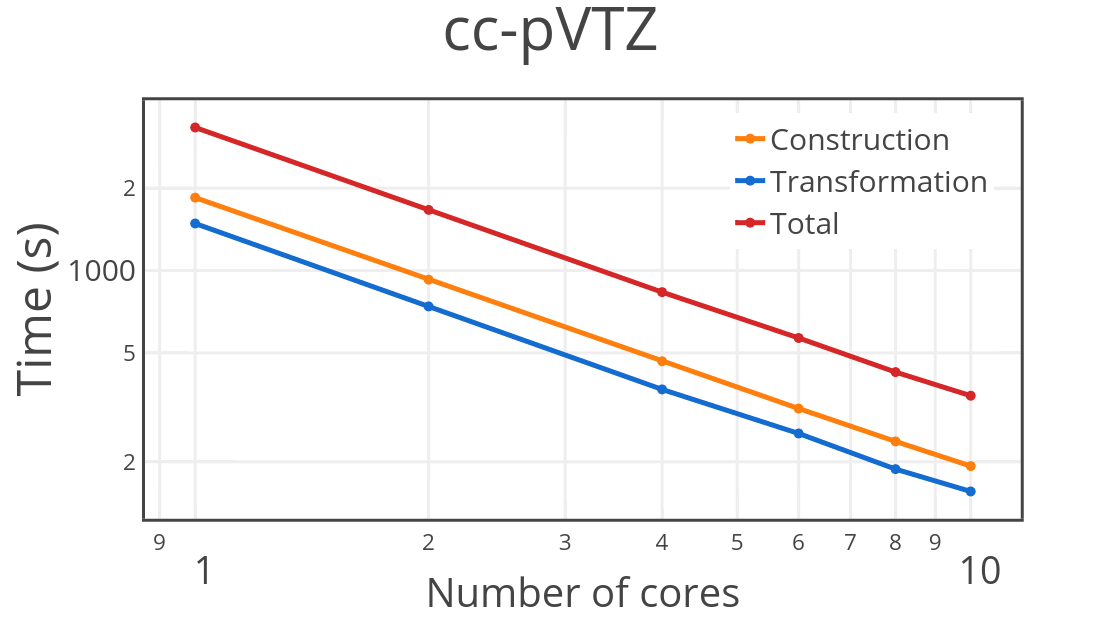
\includegraphics[width=0.5\textwidth]{figures/parallel_scaling_plots/times-cc-pVTZ.png}\label{fig:f2}}
  \hfill
  \subfloat[]{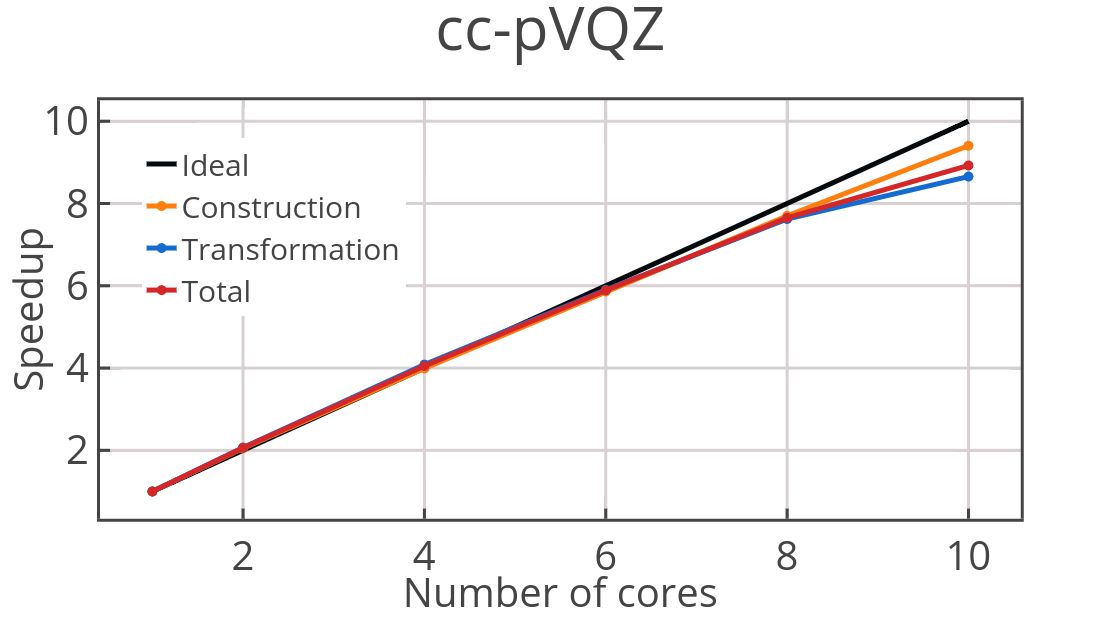
\includegraphics[width=0.5\textwidth]{figures/parallel_scaling_plots/speedup-cc-pVQZ.png}\label{fig:f1}}
  \hfill
  \subfloat[]{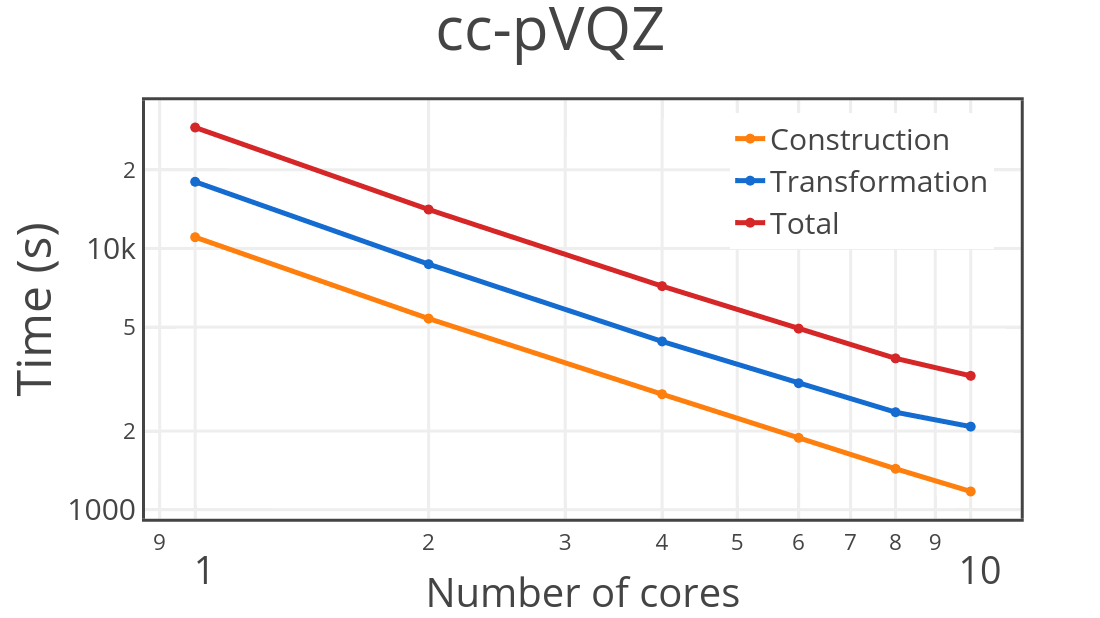
\includegraphics[width=0.5\textwidth]{figures/parallel_scaling_plots/times-cc-pVQZ.png}\label{fig:f2}}
  \hfill
  \caption{Speedup and execution time plots obtained using our optimized memory layout, $B_{\mu P \nu^\mu}$, 
 for sparsity screened 3-center integrals. 
 Execution times involve computing three common transformation classes: $(ij|Q)$, $(ib|Q)$, and $(ab|Q)$,
 where $i,j$ and $a,b$ denote occupied and virtual indices, respectively. Graphs (a), (c), and (e) include speedups for constructing the integrals (orange),
 transforming (blue), total time (red), and ideal (black). Graphs (b), (d), and (f) plot total execution times. Construction times include both integral computations
 and metric contractions. Problem sizes were increased by increasing basis set size
 using cc-pVXZ, X = D,T,Q.}
\end{figure}

At ten cores, speedups for total computation time were recorded as 9.09, 9.56, and 8.93 for $\zeta = $ D, T, Q, 
respectively. The improvement in scaling between $\zeta = $ D to $\zeta = $ T
may be attributed to larger system sizes. The sizes of the sparsity screened AO integrals were 10.38GB and 55.70GB 
for these systems, respectively. In the latter case,
the 24GB of memory at the compute node was fully used and work for each thread was increased to maximal levels. Conversely, 
when the system size was increased again using
$\zeta = $ Q, the memory constraint did not allow for further increase in work per thread. 
The hindrance in scaling from $\zeta = $ T to $\zeta = $ Q is explained by the workload imbalance incurred by
the increase in sparsity. 


\subsection{Performance Crossover Through Number of Transformations}

In this section, we reveal the contexts in which either the Store or Direct algorithms are superior. First, we analyzed performance when applying either algorithm
 to carry out each of the three common integral transformations: $(Q|ij)$, $(Q|ib)$, and $(Q|ab)$. Doing so reveals the crossover in computational complexity that occurs between the two
 algorithms. For few transformations, the Direct algorithm will be superior as it benefits from the speedups given
 in Table 3.2. However, if many transformations occur, we propose the Store algorithm will become superior as it avoids the costly metric contraction for each transformation.
 
We applied both algorithms to each transformation using the
same boron catalyst system in Figure 3.1. To reveal the crossover in computational work between the two algorithms, 
the execution times to carry out one to ten transformations were recorded. To reveal additional trends, we varied the
system size by adjusting the basis set size using $\zeta$ = D, T, Q. The characteristics of these systems are described in Table 3.3.
The experiments were carried out using one node consisting of an Intel Core i7-5930K processor
(6 cores at 3.50GHz) and 50GB DRAM. The results are plotted in Figure 3.3.
 
\begingroup
\begin{table}[H]
\centering
\renewcommand{\baselinestretch}{1}
\caption{Characteristics of organoboron catalyst systems across the cc-pVDZ, cc-pVTZ, and cc-pVQZ basis sets.}
\begin{tabular}{l cccc}
\multicolumn{1}{l}{\textbf{Basis}} &
\multicolumn{1}{c}{\textbf{$N_{AO}$}} &
\multicolumn{1}{c}{\textbf{$N_{aux}$}} &
\multicolumn{1}{c}{\textbf{$N_{occ}$}} &
\multicolumn{1}{c}{\textbf{$N_{virt}$}} \\
\hline
cc-pVDZ   & 671  & 3277      & 129       & 542        \\ 
cc-pVTZ   & 1566 & 3856      & 129       & 1437       \\ 
cc-pVQZ   & 3040 & 5593      & 129       & 2911       \\ 
\end{tabular}
\end{table}
\endgroup

\begin{figure}[H]
  \captionsetup[subfigure]{labelformat=empty}
  \centering
  \subfloat[]{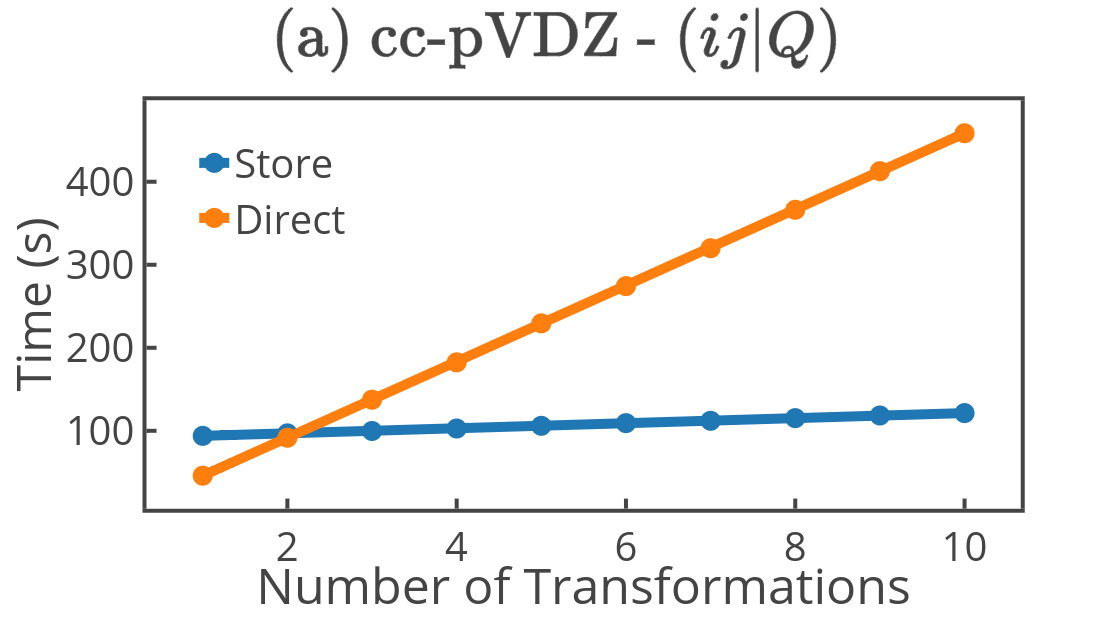
\includegraphics[width=0.35\textwidth]{figures/workflow_plots/input1-cc-pVDZ.png}}
  %\hfill
  \subfloat[]{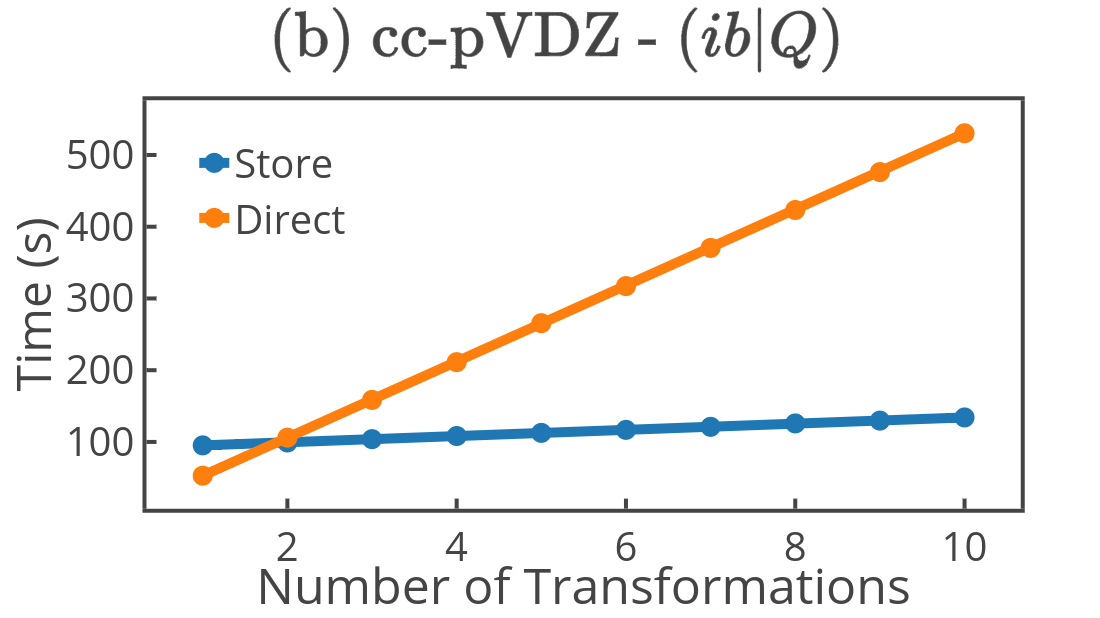
\includegraphics[width=0.35\textwidth]{figures/workflow_plots/input2-cc-pVDZ.png}}
  %\hfill
  \subfloat[]{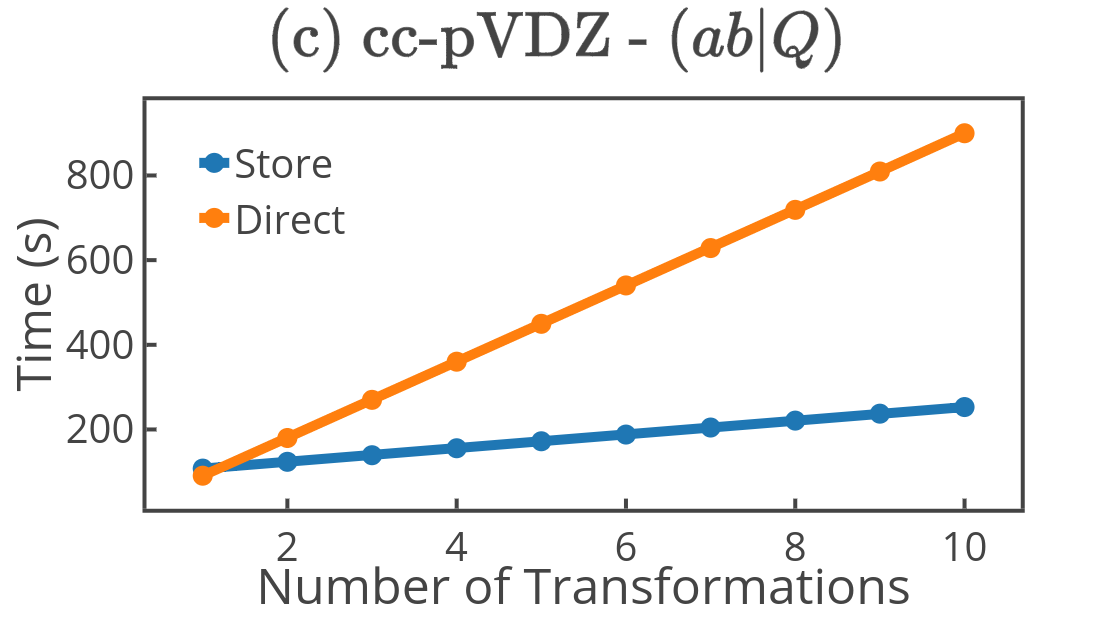
\includegraphics[width=0.35\textwidth]{figures/workflow_plots/input3-cc-pVDZ.png}}\\[-4ex]
  \hfill
  \subfloat[]{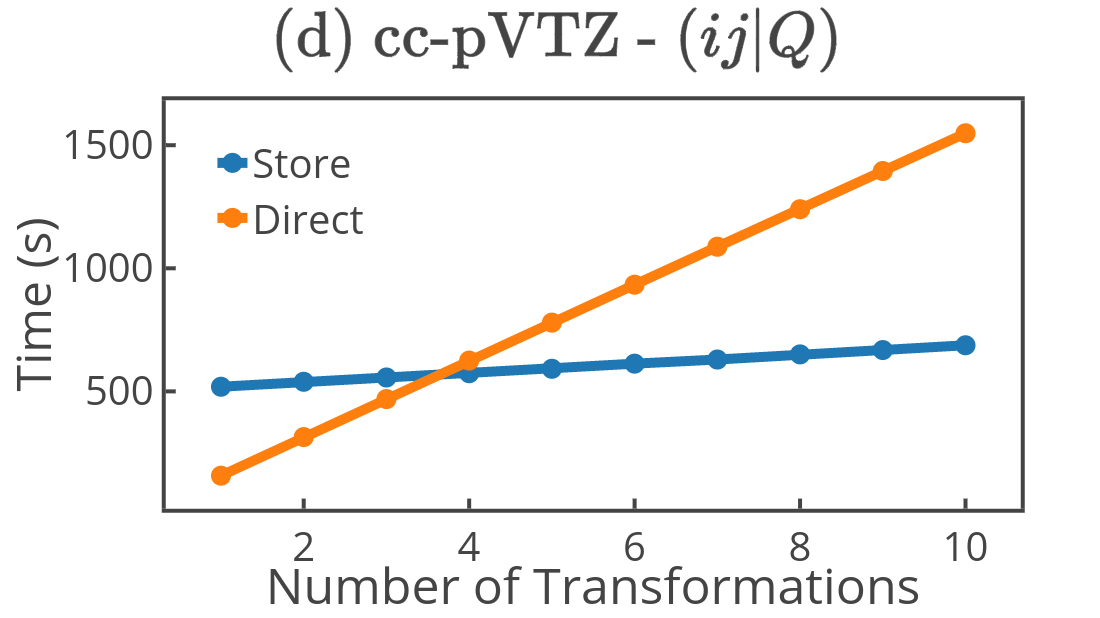
\includegraphics[width=0.35\textwidth]{figures/workflow_plots/input1-cc-pVTZ.png}}
  %\hfill
  \subfloat[]{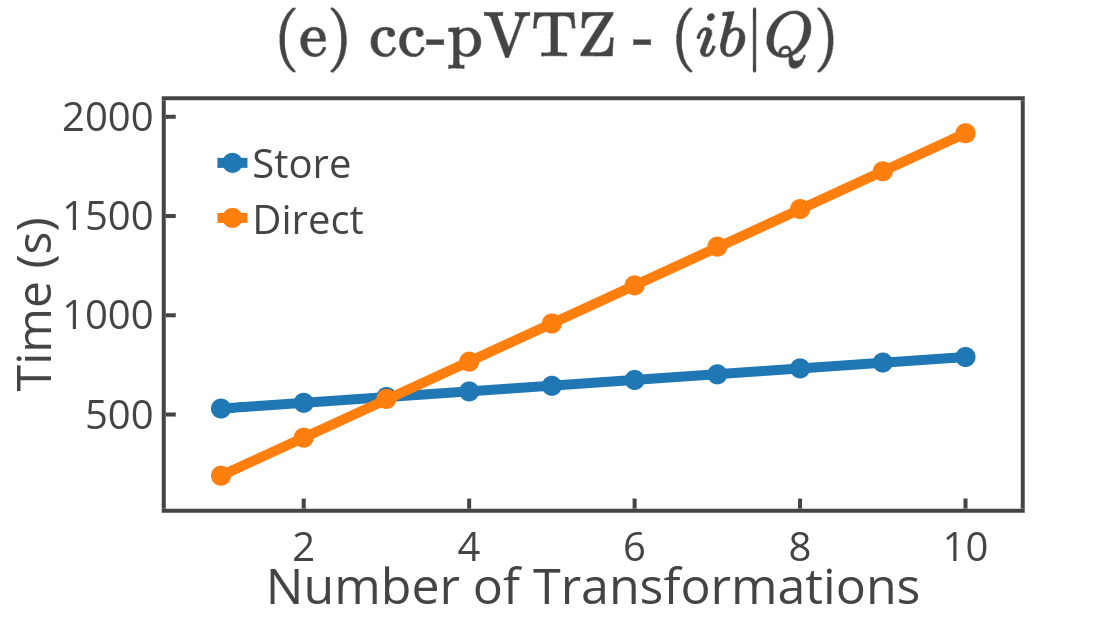
\includegraphics[width=0.35\textwidth]{figures/workflow_plots/input2-cc-pVTZ.png}}
  %\hfill
  \subfloat[]{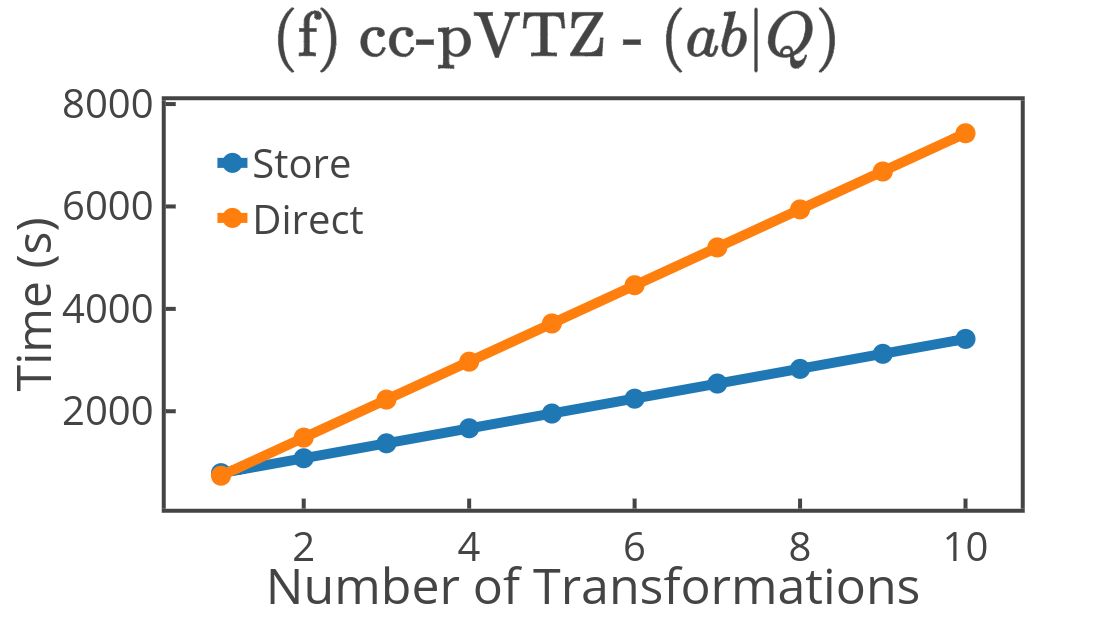
\includegraphics[width=0.35\textwidth]{figures/workflow_plots/input3-cc-pVTZ.png}}\\[-4ex]
  \hfill
  \subfloat[]{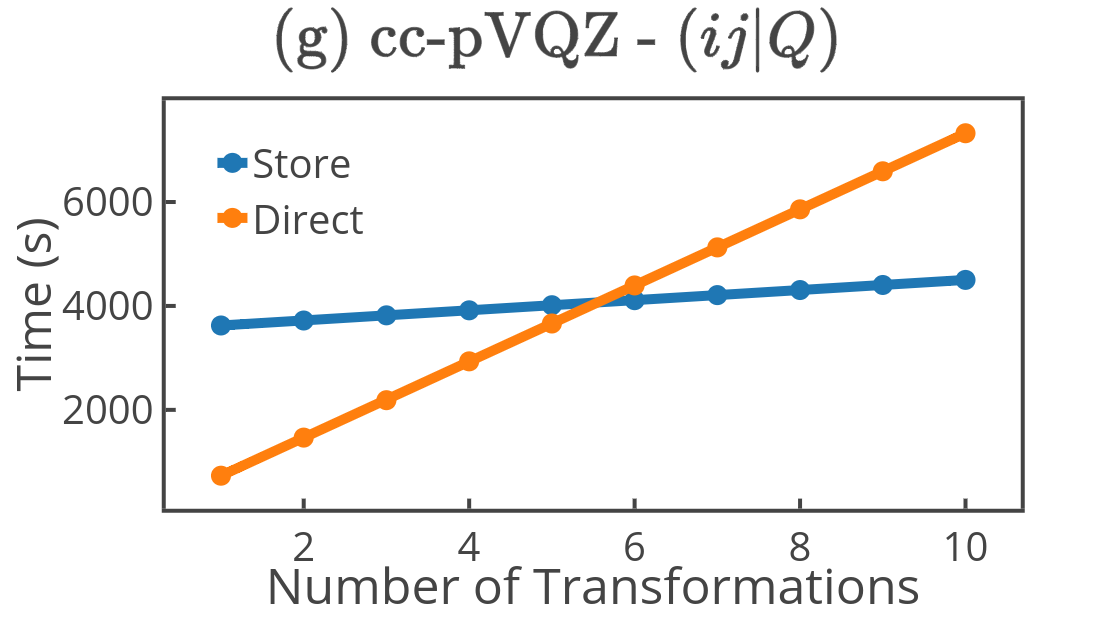
\includegraphics[width=0.35\textwidth]{figures/workflow_plots/input1-cc-pVQZ.png}}
  %\hfill
  \subfloat[]{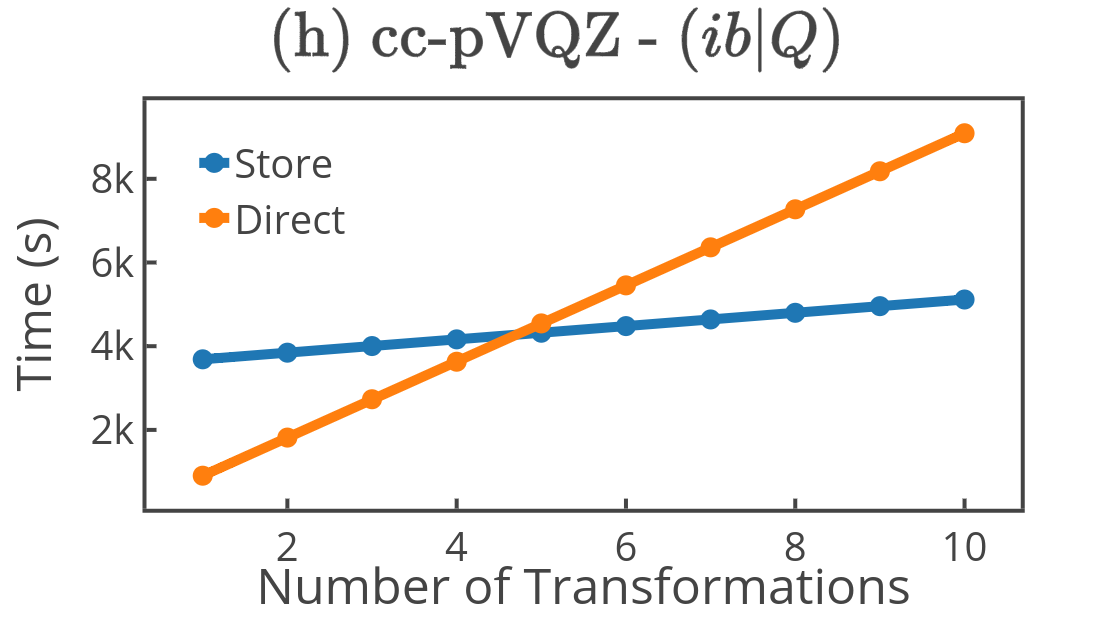
\includegraphics[width=0.35\textwidth]{figures/workflow_plots/input2-cc-pVQZ.png}}
  %\hfill
  \subfloat[]{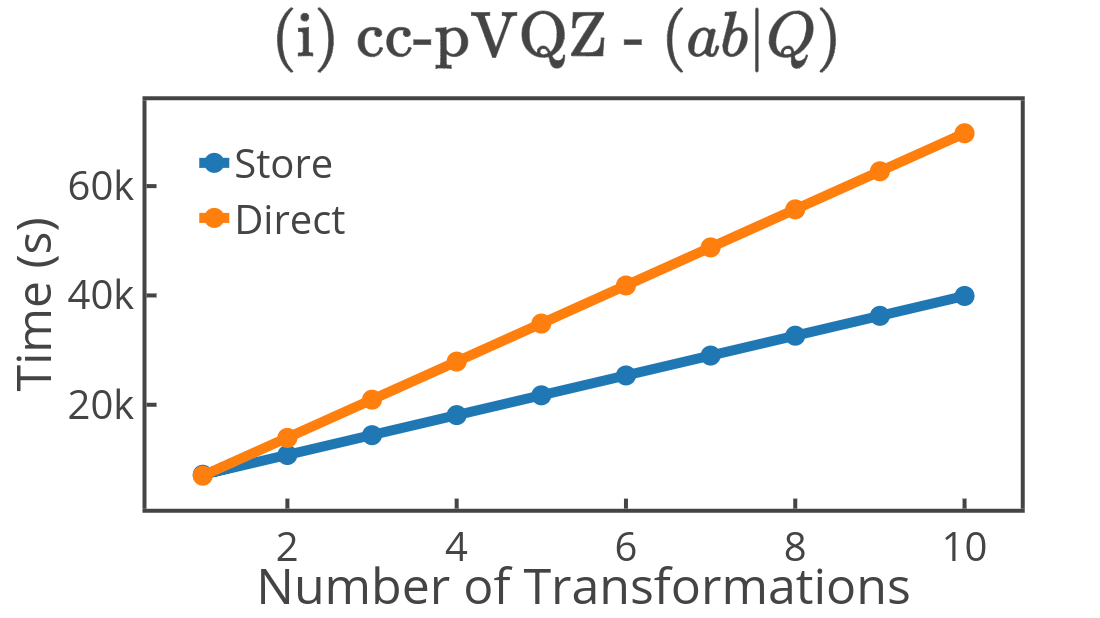
\includegraphics[width=0.35\textwidth]{figures/workflow_plots/input3-cc-pVQZ.png}}
  \caption{Comparison of total execution times for the Store and Direct algorithms to complete $(ij|Q)$, $(ib|Q)$, and $(ab|Q)$ transformations
across the cc-pVDZ, cc-pVTZ, and cc-pVQZ basis sets. A scan from one to ten transformations was performed. In each case, a crossover
occurs as the Direct algorithm becomes more expensive. The crossover occurs in fewer iterations for transformations involving larger MO spaces.
With increasing basis set size, the crossover point is shifted to the right for the $(ij|Q)$ and $(ib|Q)$
transformations and it is shifted slightly to the left for the $(ab|Q)$ transformation.}
\end{figure}

If only one transformation occurs, then the speedups of Table 3.2 enable the Direct algorithm to be superior. 
However, the Direct algorithm must carry out expensive metric contractions for every transformation. As the
number of transformations increase, the expense of these contractions
overtakes the speedups of pre-transforming the integrals. Note that a crossover between the two algorithms occurs in each system. 
This finding supports our conjecture that the Store algorithm is advantageous in contexts where many transformations occur. 
This includes iterative methods where the transformations
are carried out in each iteration, such as MCSCF, as well as methods which require many transformations, such as SAPT.
Conversely, the Direct algorithm is advantageous for methods
requiring few transformations, such as DFMP2.

Additionally, the crossover point shifts to the left as the transformation spaces get larger ($ij, ia, ab$), occurring in fewer transformations.
This finding is supportive of the proposed speedups in Table 3.2.
Therefore procedures using anything larger than a $(ib|Q)$ transformation will receive nominal benefits from employing the 
Direct algorithm and may incur slowdowns if many transformations occur.
Last, the crossover point shifts to the right for the $(ij|Q)$ and $(ib|Q)$ transformations as larger basis sets are used. 
This will allow for 
continued benefits with more transformations. Conversely, the crossover shifts to the left for the $(ab|Q)$ transformation
for larger basis sets. Either of these findings are elucidated
by the increasing ratio of $\frac{N_{aux}}{N_{AO}}$. 
 

\subsection{Superior Workflows in Practice}

In the previous section, we determined the Direct algorithm will be superior in methods such as DFMP2, while the Store 
algorithm will be superior in methods such as MCSCF.
After determining the contexts in which either algorithm prevail, we sought to reveal their benefits when applied in practice. 
To do so, we employed either algorithm
in the contexts of different procedures and systems. For procedures, we tested DFMCSCF and DFMP2. We ran these 
procedures on the systems included in Figure 3.4.
Figure 3.4 (a) is a hexatriene molecule. Figure 3.4 (b) is benzene and toluene solvated by 20 water molecules.
Table 3.4 lists the characteristics of each system,
which includes the basis set, the number of primary and auxiliary basis functions, and the mask sparsity. 


\begin{figure}[H]
  \captionsetup[subfigure]{}
  \centering
  \subfloat[]{\includegraphics[width=55mm]{geometries/hexatriene.png}}
  \subfloat[]{\includegraphics[width=55mm]{geometries/benzene-toluene-solvated.png}} 
  \hfill
  \caption{Systems used for context dependent investigation of the Store and Direct workflows. (a) Hexatriene. (b) Benzene and toluene 
in 20 water solvent molecules. }
\end{figure}

\begingroup
\begin{table}[H]
\centering
\renewcommand{\baselinestretch}{1}
\caption{Characteristics of systems for Store vs Direct algorithm comparisons.}
\begin{tabular}{l ccccc}
\multicolumn{1}{l}{\textbf{System}} &
\multicolumn{1}{c}{\textbf{Primary Basis}} &
\multicolumn{1}{c}{\textbf{Auxiliary Basis}} &
\multicolumn{1}{c}{\textbf{$N_{aux}$}} &
\multicolumn{1}{c}{\textbf{$N_{virt}$}} \\
\hline
Hexatriene        & cc-pVQZ     & cc-pVQZ-jkfit     & 570   &  1044        \\ 
Hexatriene        & cc-pVQZ     & cc-pVQZ-rifit     & 570   &  1232        \\ 
Benzene-Toluene   & jun-cc-pVDZ & jun-cc-pVDZ-jkfit & 867   &  3849       \\ 
Benzene-Toluene   & jun-cc-pVDZ & jun-cc-pVDZ-rifit & 867   &  2901       \\ 
\end{tabular}
\end{table}
\endgroup

The experiments were carried out using one node consisting of an Intel Core i7-5930K processor
(6 cores at 3.50GHz) and 60GB DRAM. The results are included in Tables 3.6 and 3.7. Table 3.6 includes
the total computation time spent in operations involving the three-index integrals. These times will
reflect the algorithmic benefits illustrated in Figure 3.3. Table 3.7 includes the total time required
to execute the program. These times reflect total procedure times, which include many operations extraneous
to the three-index integrals.

\begingroup
\begin{table}[H]
\centering
\renewcommand{\baselinestretch}{1}
\caption{Computational times comparing the Direct and Store algorithms for three-index integral construction and
transformations.}
\begin{tabular}{l cccc}
\multicolumn{1}{l}{\textbf{System}} &
\multicolumn{1}{c}{\textbf{Procedure}} &
\multicolumn{1}{c}{\textbf{DIRECT}} &
\multicolumn{1}{c}{\textbf{STORE}} &
\multicolumn{1}{c}{\textbf{Speedup}} \\ 
\hline
Hexatriene        & DFMCSCF & 42.3s   &   7.8s  &  5.4x  \\ 
Hexatriene        & DFMP2   &  2.9s   &   6.0s  &  2.1x  \\ 
Benzene-Toluene   & DFMCSCF & 438.1s  & 104.8s  &  4.2x  \\ 
Benzene-Toluene   & DFMP2   & 31.4s   &  61.2s  &  1.9x  \\ 
\end{tabular}
\end{table}
\endgroup


\begingroup
\begin{table}[H]
\centering
\renewcommand{\baselinestretch}{1}
\caption{Total procedure wall clock times comparing the Direct and Store algorithms.}
\begin{tabular}{l cccc}
\multicolumn{1}{l}{\textbf{System}} &
\multicolumn{1}{c}{\textbf{Procedure}} &
\multicolumn{1}{c}{\textbf{DIRECT}} &
\multicolumn{1}{c}{\textbf{STORE}} &
\multicolumn{1}{c}{\textbf{Speedup}} \\ 
\hline
Hexatriene        & DFMCSCF & 173.0s   & 145.6s  &  1.2x  \\ 
Hexatriene        & DFMP2   & 35.1s    &  40.5s  &  1.2x  \\ 
Benzene-Toluene   & DFMCSCF & 5138.7s  & 4811.8s &  1.1x  \\ 
Benzene-Toluene   & DFMP2   & 852.7s   & 856.0s  &  1.0x  \\ 
\end{tabular}
\end{table}
\endgroup

Both Tables 3.6 and 3.7 reveal that the Direct algorithm is superior for DFMP2 whereas the Store algorithm is superior for
DFMCSCF. The computational speedups can be substantial, reaching 5.4x for DFMCSCF with the hexatriene system. However, Table 3.7
reveals these speedups are considerably dampened for the overall procedure time. This is true because 
the operations involving the three-index integrals are not the most expensive computations occurring within these procedures.



